\begin{document}
%=================================================================
%                           Start Document
%=================================================================
\sectiontitle{4}{Theory}


\lhead{Theory - Functional Electrical Stimulation} % section header

\setstretch{1.6}

\subsection{Functional Electrical Stimulation}
Functional Electrical stimulation (FES) is the application of electrical current to excitable tissue to supplement or replace a function that is lost in neurologically impaired individuals. FES can be used for chronic applications for restoration of function or in therapeutic applications as it is used in the project. The aim of therapeutic electrical stimulation is to improve tissue health or voluntary function by inducing physiological changes that remain after the stimulation. 

Stimulation is delivered as a waveform of electrical current pulses, which are characterized by three parameters: pulse frequency, amplitude and duration, as well as the shape of the pulse train. The strength of the muscle contraction is determined by modulating these parameters.

\begin{figure} [H]
    \centering
    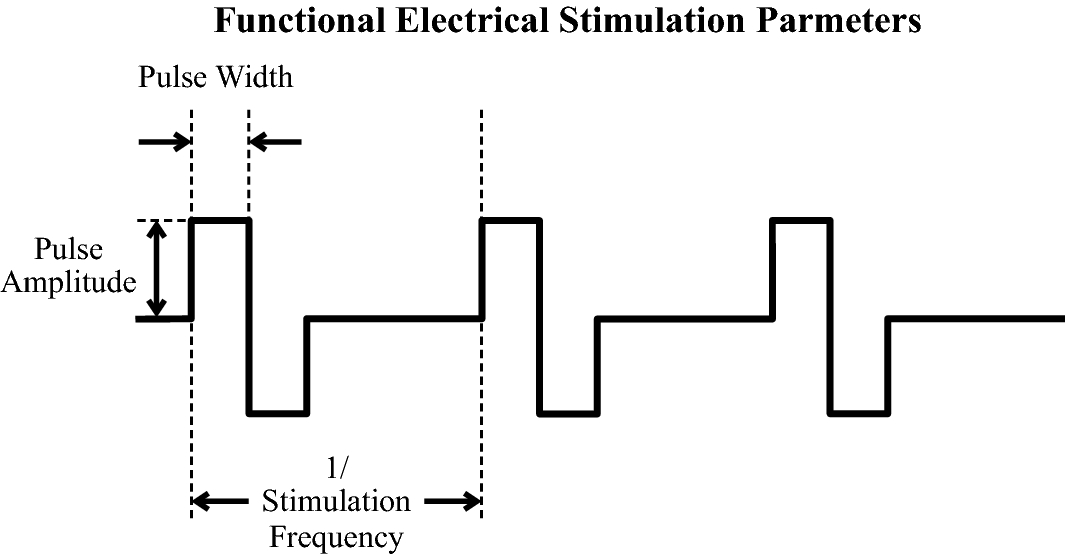
\includegraphics[width=0.7\linewidth]{images/stimpar.png}
    \caption{Illustration of a typical biphasic stimulation waveform and its parameters \cite{marquez-chin_functional_2020}}
    \label{fig:waveforms}
\end{figure}

The resulting torque about the joint that is actuated by the muscle depends on the tension in the flexor and extensor muscles as well as the biomechanics of the joint \cite{lynch_functional_2008}. 


FES recruits motor units in a synchronous manner, unlike an intact nervous system that recruits in an asynchronously. Thus FES requires a much higher stimulation frequency (20-40Hz), compared to the typical nervous system frequency (6-8Hz) in order to achieve sustained muscle contraction \cite{lynch_functional_2008}. This is the main cause of the increased rate of fatigue associated with FES contraction as compared to contraction initiated by the central nervous system (CNS) \cite{gilman_handbook_1983}. 

Furthermore FES is believed to recruit the fast-twitch fibers before the slow-twitch fibers, due to the larger diameter of innervation axons. This non-physiological recruitment is the opposite of natural muscle-fiber recruitment order.Since fast-twitch fibers fatigue more quickly than slow twitch fibers, this also leads to the increased fatigue seen with artificial stimulation. \cite{lynch_functional_2008}

When an artificially stimulated muscle begins to fatigue, its response changes non-linearly \cite{lynch_functional_2008}, and will eventually stop contracting. 

FES applications for motor function uses the fundamental principle that electrical stimulation generally activates nerve rather than muscle \cite{peckham_functional_2005}. This is because the threshold charge for directly eliciting muscle fiber action potentials is much greater than the threshold of producing action potentials in neurons. Thus for FES to be effective, the lower motor neurons must be intact from the anterior horns of the spinal cord to the neuromuscular junctions in the muscles that , as is usually the case with spinal cord injury, stroke, head injuries, cerebral palsy and multiple sclerosis \cite{gregory_recruitment_2005}. 

\lhead{Theory - Gait Phases}
\subsection{Gait Phases}
The gait cycle is traditionally divided into two primary phases: the stance phase, when the foot is in contact with the ground, and the swing phase, when the foot is off the ground. These phases, in turn, can be broken down into sub-phases that describe distinct biomechanical and functional tasks. A clear understanding of these phases is crucial for effective application of FES in gait rehabilitation.

\begin{figure}
    \centering
    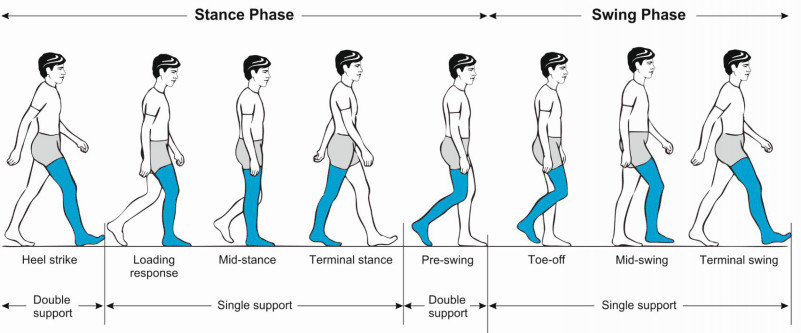
\includegraphics[width=0.9\linewidth]{images/Phases-of-the-normal-gait-cycle.png}
    \caption{Gait Phases \cite{pirker_gait_2017}}
    \label{fig:enter-label}
\end{figure}

The stance phase constitutes approximately 60\% of the gait cycle and begins with initial contact, where the heel first strikes the ground. This moment marks the beginning of weight acceptance and serves to provide stability and absorb shock. Following initial contact, the loading response occurs as the body transfers weight onto the limb, with both feet briefly in contact with the ground. During mid-stance, the body progresses over the supporting limb resting in a period of single-limb support. As the body continues to move forward, terminal stance begins, characterized by the heel rising off the ground and the weight shifting towards the forefoot. The final sub-phase of stance, pre-swing, occurs as the toes push off the ground, preparing the limb for the swing phase. During this phase, the gluteus maximus and quadriceps are essential for maintaining hip and knee stability, while the gastrocnemius and soleus muscles begin to engage for forward propulsion.

The swing phase, which occupies the remaining 40\% of the gait cycle, involves the limb moving forward while the foot remains off the ground. his phase begins with initial swing, during which the foot is lifted from the ground through the combined action of the hip flexors and knee flexors, particularly the hamstrings. The tibialis anterior is re-engaged to maintain dorsiflexion and prevent toe drag. During mid-swing, the limb continues its forward trajectory, with the hip flexors and dorsiflexors ensuring sufficient clearance and alignment for the upcoming stance phase. Finally, terminal swing occurs as the limb decelerates, relying on the hamstrings to control knee extension and the gluteus maximus to stabilize the hip. The limb prepares for the next initial contact, ensuring proper positioning for stability and weight acceptance.

Each sub-phase of the gait cycle plays a critical role in maintaining balance, propulsion, and efficiency during walking. Disruptions in these phases, such as those caused by neurological impairments, can lead to abnormal gait patterns.






%=================================================================
%                           End Document
%=================================================================
\end{document}